\section{Supplementary results}
\label{app:tables}

\subsection{The endpoint on every instrument, all four arms}

\begin{table*}[h]
\centering
\small
\setlength{\tabcolsep}{5pt}
\begin{tabular}{@{}lrrrr@{}}
\toprule
& \PTO\ $\Kz$ & \PTO\ $\Kf$ & \GRPO\ $\Kz$ & \GRPO\ $\Kf$\\
\midrule
\multicolumn{5}{@{}l}{\emph{\primaryjudge\ (training oracle)}}\\
Q1+Q2 (reward)  & $4.260$ ($+1.259$) & $4.307$ ($+1.304$) & $3.753$ ($+0.686$) & $4.517$ ($+1.554$)\\
\quad Q1        & $4.140$ ($+1.217$) & $4.225$ ($+1.279$) & $3.606$ ($+0.585$) & $4.465$ ($+1.554$)\\
\quad Q2        & $4.380$ ($+1.302$) & $4.388$ ($+1.328$) & $3.899$ ($+0.786$) & $4.570$ ($+1.554$)\\
WAI-SR          & $3.497$ ($+0.653$) & $3.536$ ($+0.716$) & $3.438$ ($+0.549$) & $3.729$ ($+0.872$)\\
CSQ-8           & $2.945$ ($+0.561$) & $2.953$ ($+0.615$) & $2.773$ ($+0.411$) & $3.062$ ($+0.707$)\\
MI-SAT          & $3.653$ ($+0.816$) & $3.710$ ($+0.872$) & $3.479$ ($+0.622$) & $3.832$ ($+1.016$)\\
MITI            & $4.273$ ($+1.141$) & $4.258$ ($+1.109$) & $3.922$ ($+0.698$) & $4.537$ ($+1.417$)\\
PCT             & $0.630$ ($+0.141$) & $0.638$ ($+0.156$) & $0.574$ ($+0.087$) & $0.685$ ($+0.214$)\\
MICI ($\downarrow$) & $0.491$ ($+0.278$) & $0.264$ ($+0.086$) & $0.838$ ($+0.626$) & $0.210$ ($+0.002$)\\
\addlinespace
\multicolumn{5}{@{}l}{\emph{\heldoutjudge\ (held out)}}\\
Q1+Q2 (reward)  & $2.866$ ($+1.036$) & $2.667$ ($+0.833$) & $2.257$ ($+0.396$) & $2.873$ ($+1.038$)\\
\quad Q1        & $2.640$ ($+0.967$) & $2.604$ ($+0.921$) & $1.867$ ($+0.173$) & $2.731$ ($+1.050$)\\
\quad Q2        & $3.092$ ($+1.106$) & $2.730$ ($+0.746$) & $2.648$ ($+0.620$) & $3.015$ ($+1.027$)\\
WAI-SR          & $2.955$ ($+0.838$) & $2.851$ ($+0.701$) & $2.669$ ($+0.447$) & $2.958$ ($+0.792$)\\
CSQ-8           & $2.809$ ($+0.767$) & $2.807$ ($+0.708$) & $2.484$ ($+0.397$) & $2.935$ ($+0.844$)\\
MI-SAT          & $3.073$ ($+0.609$) & $3.184$ ($+0.721$) & $2.825$ ($+0.304$) & $3.328$ ($+0.889$)\\
MITI            & $2.352$ ($+0.513$) & $2.148$ ($+0.297$) & $2.099$ ($+0.211$) & $2.375$ ($+0.544$)\\
PCT             & $0.633$ ($+0.113$) & $0.685$ ($+0.161$) & $0.613$ ($+0.087$) & $0.725$ ($+0.219$)\\
MICI ($\downarrow$) & $0.825$ ($+0.461$) & $0.581$ ($+0.210$) & $1.050$ ($+0.666$) & $0.628$ ($+0.301$)\\
\bottomrule
\end{tabular}
\caption{Iteration-10 mean over the 96 personas for every arm $\times$ instrument, with the gain
over that arm's own base in parentheses. Every own-base gain is Holm-significant at $p < .01$
except \GRPO-$\Kf$'s MICI (a \emph{flat} line, $+0.002$, $p = .71$ --- the training oracle
reading no drift) and \PTO-$\Kf$'s MICI under the training oracle ($+0.086$, $p = .002$). Levels
are in each grader's own units; the two blocks are never compared to each other. MICI is
lower-is-better, so a \emph{small} gain is good on that row.}
\label{tab:endpoints}
\end{table*}

\begin{figure*}[h]
\centering
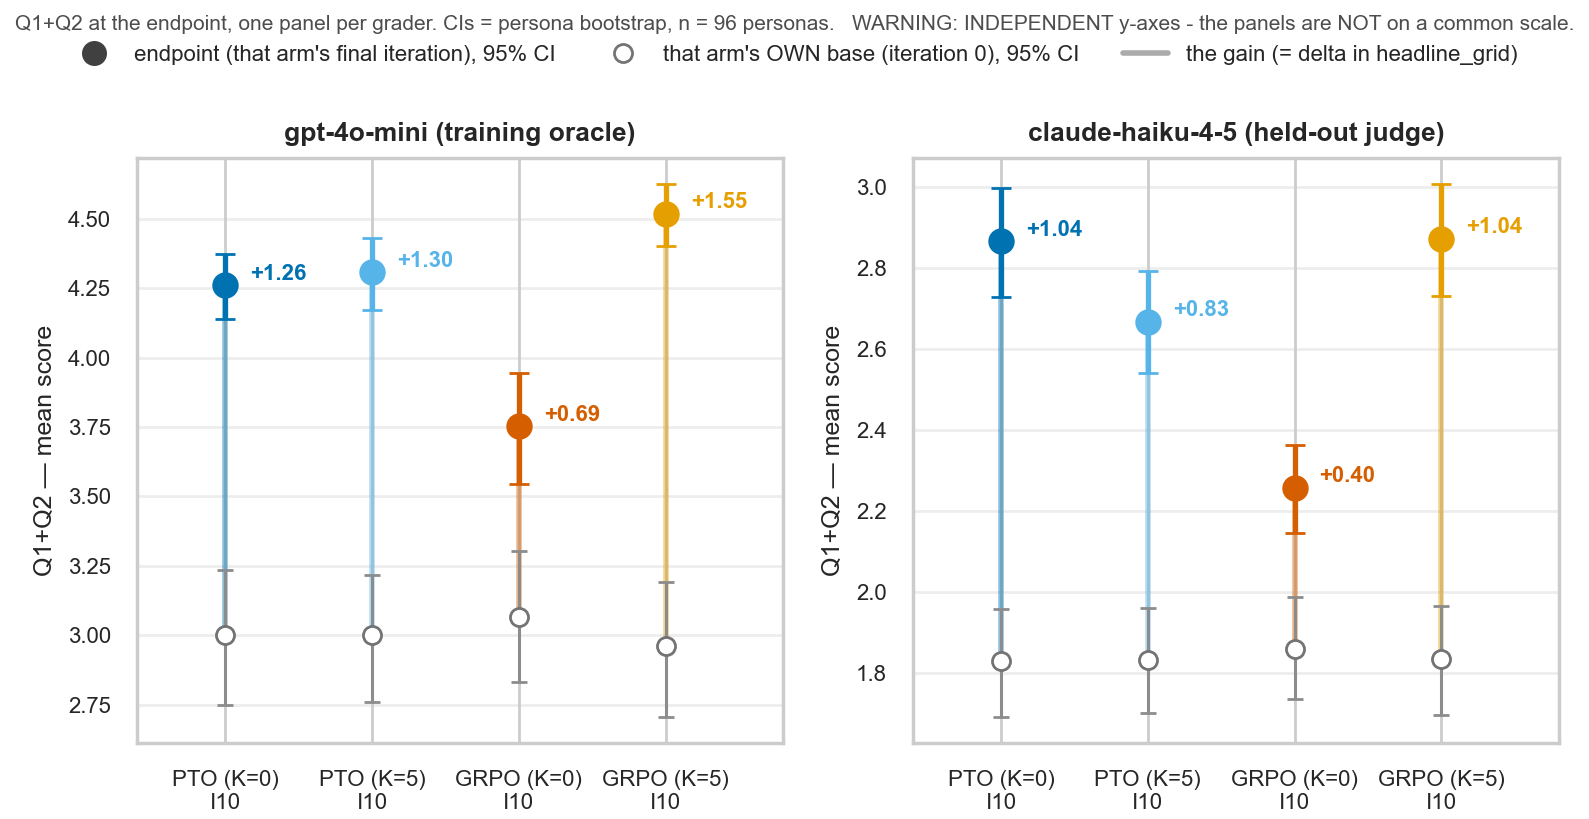
\includegraphics[width=0.9\textwidth]{figures/headline_grid.png}
\caption{The endpoint grid as a figure: all four arms under both graders, each arm anchored to
its own base. The panels are not on a common scale.}
\label{fig:headlinegrid}
\end{figure*}

\subsection{Per-channel behaviour forests}

\begin{figure*}[h]
\centering
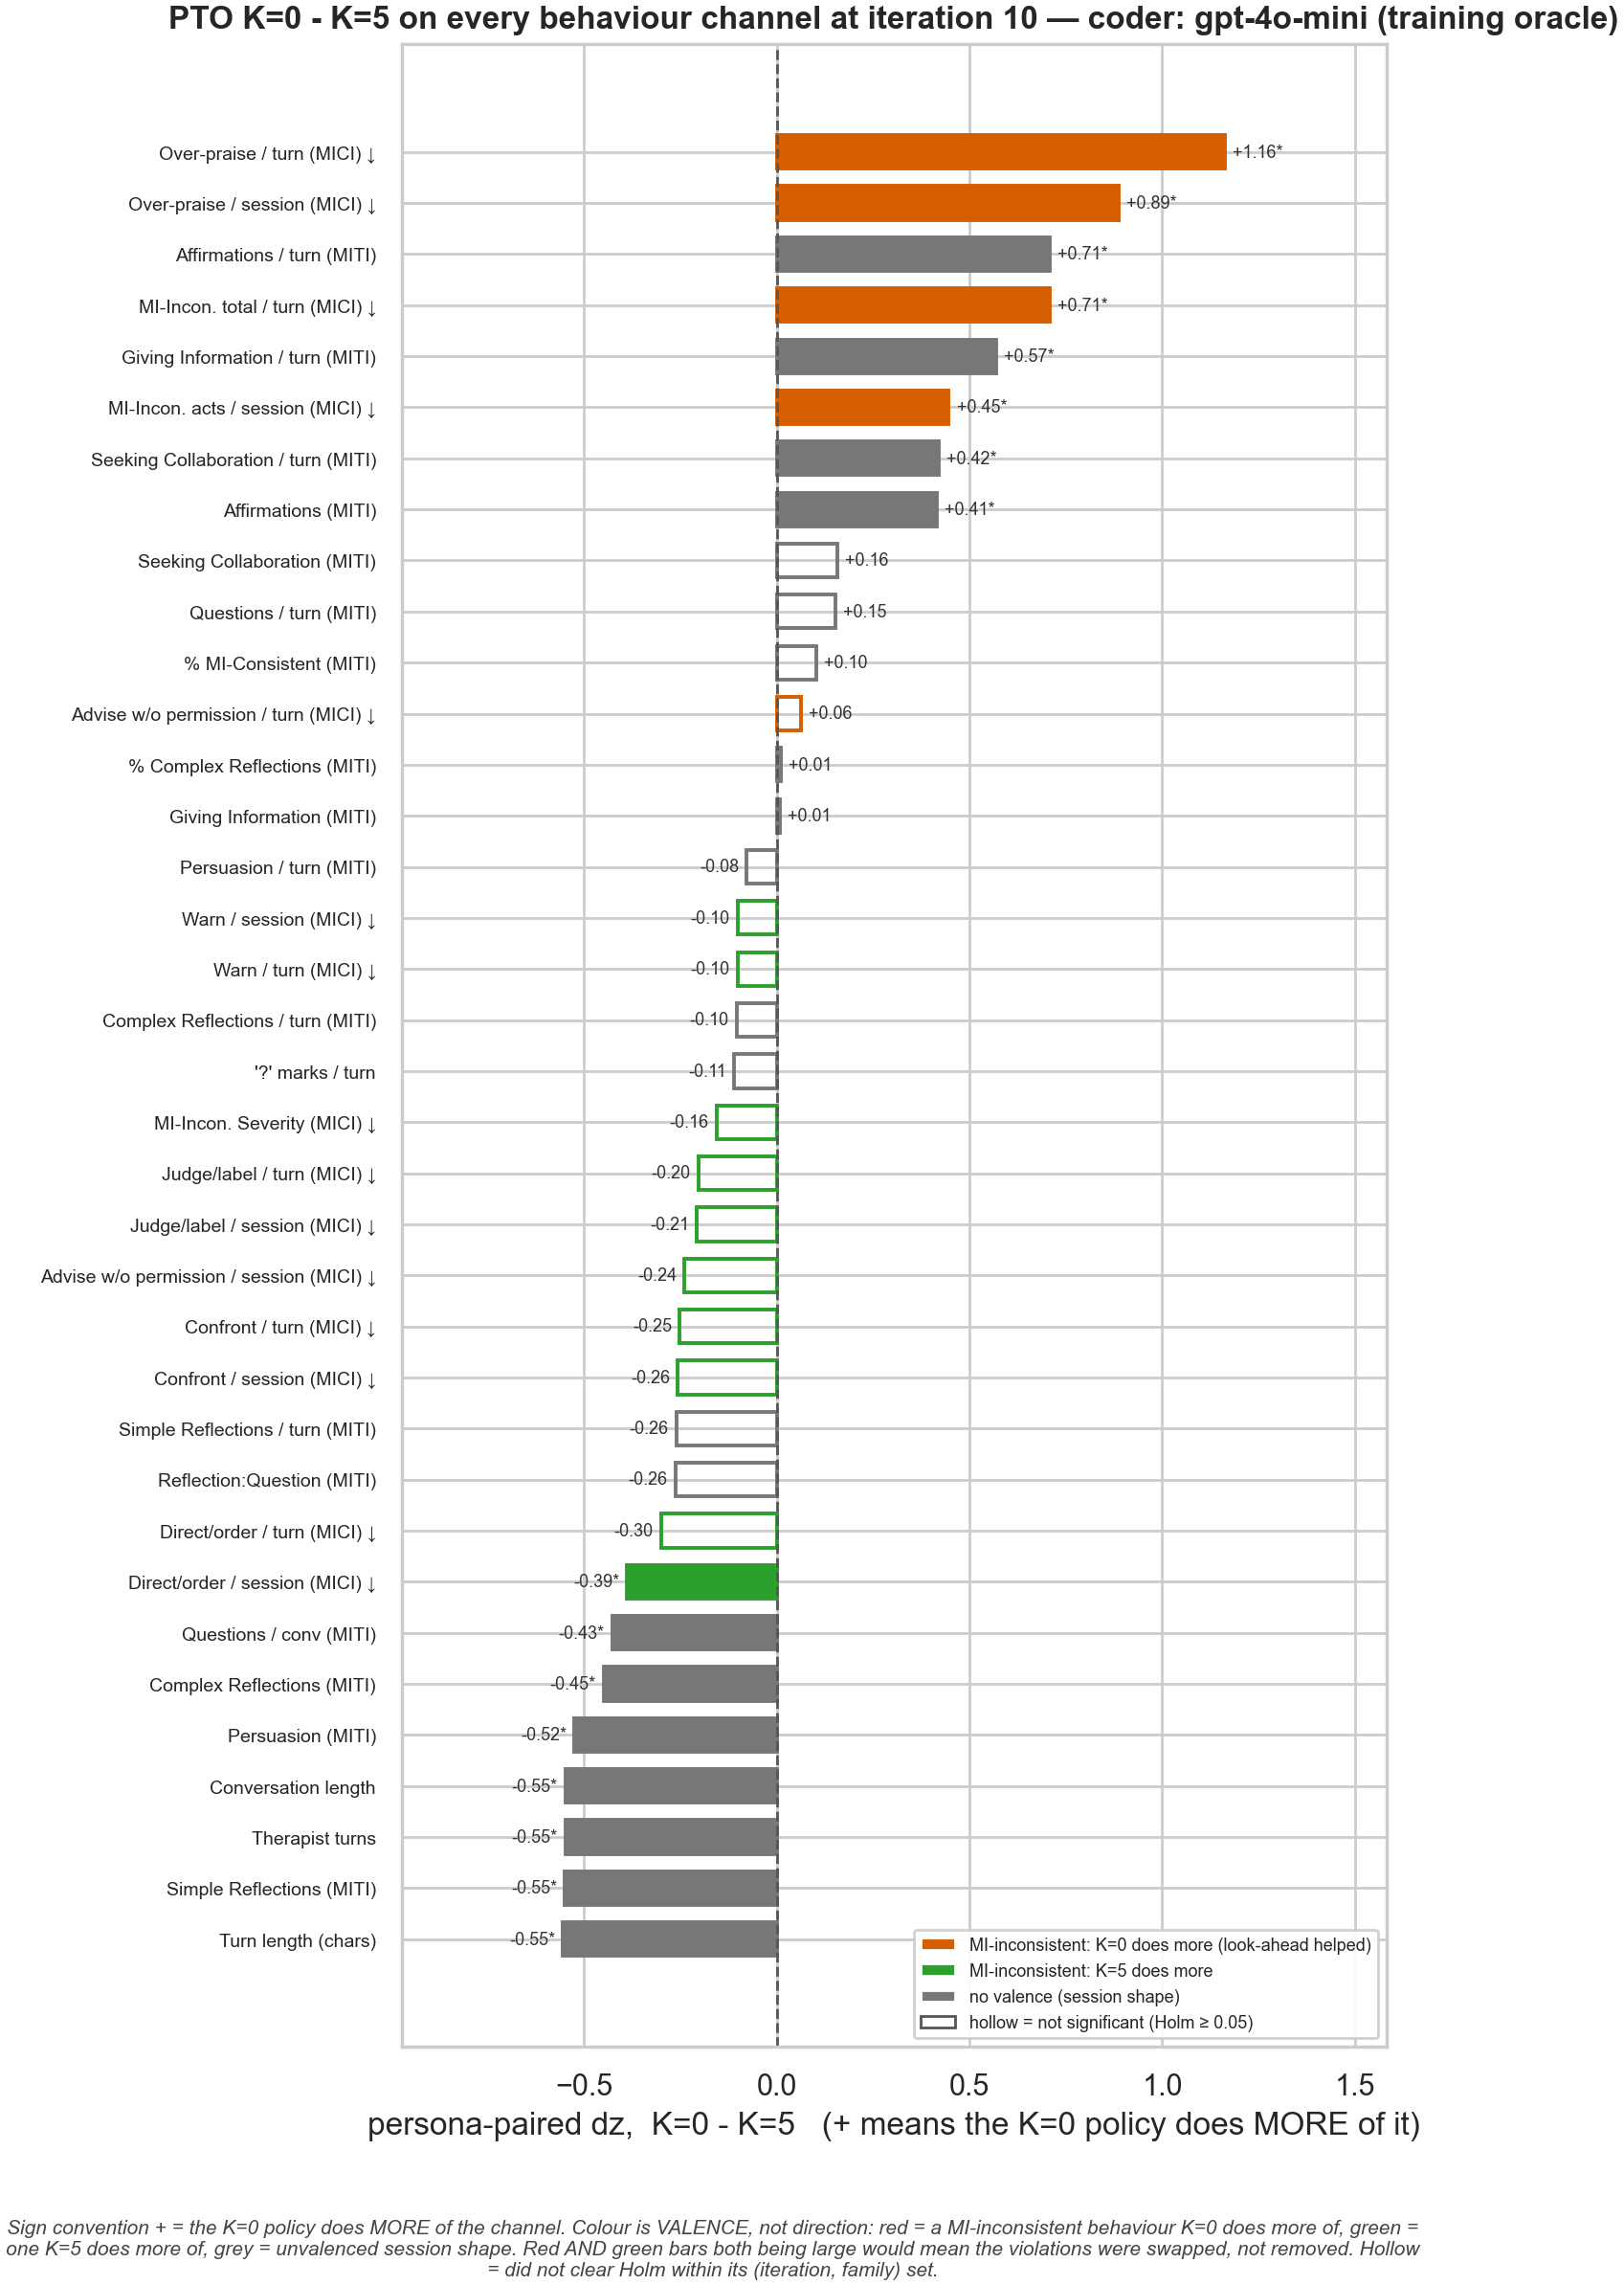
\includegraphics[width=0.85\textwidth]{figures/k_channel_forest_pto_gpt-4o-mini.png}
\caption{\PTO: every behaviour channel's persona-paired \dz\ at the endpoint under the training
oracle (positive = the $\Kz$ policy does more; colour = valence; hollow = failed Holm).
Over-praise (red) closes under $\Kf$ while advice-without-permission (green) opens --- the
substitution.}
\end{figure*}

\begin{figure*}[h]
\centering
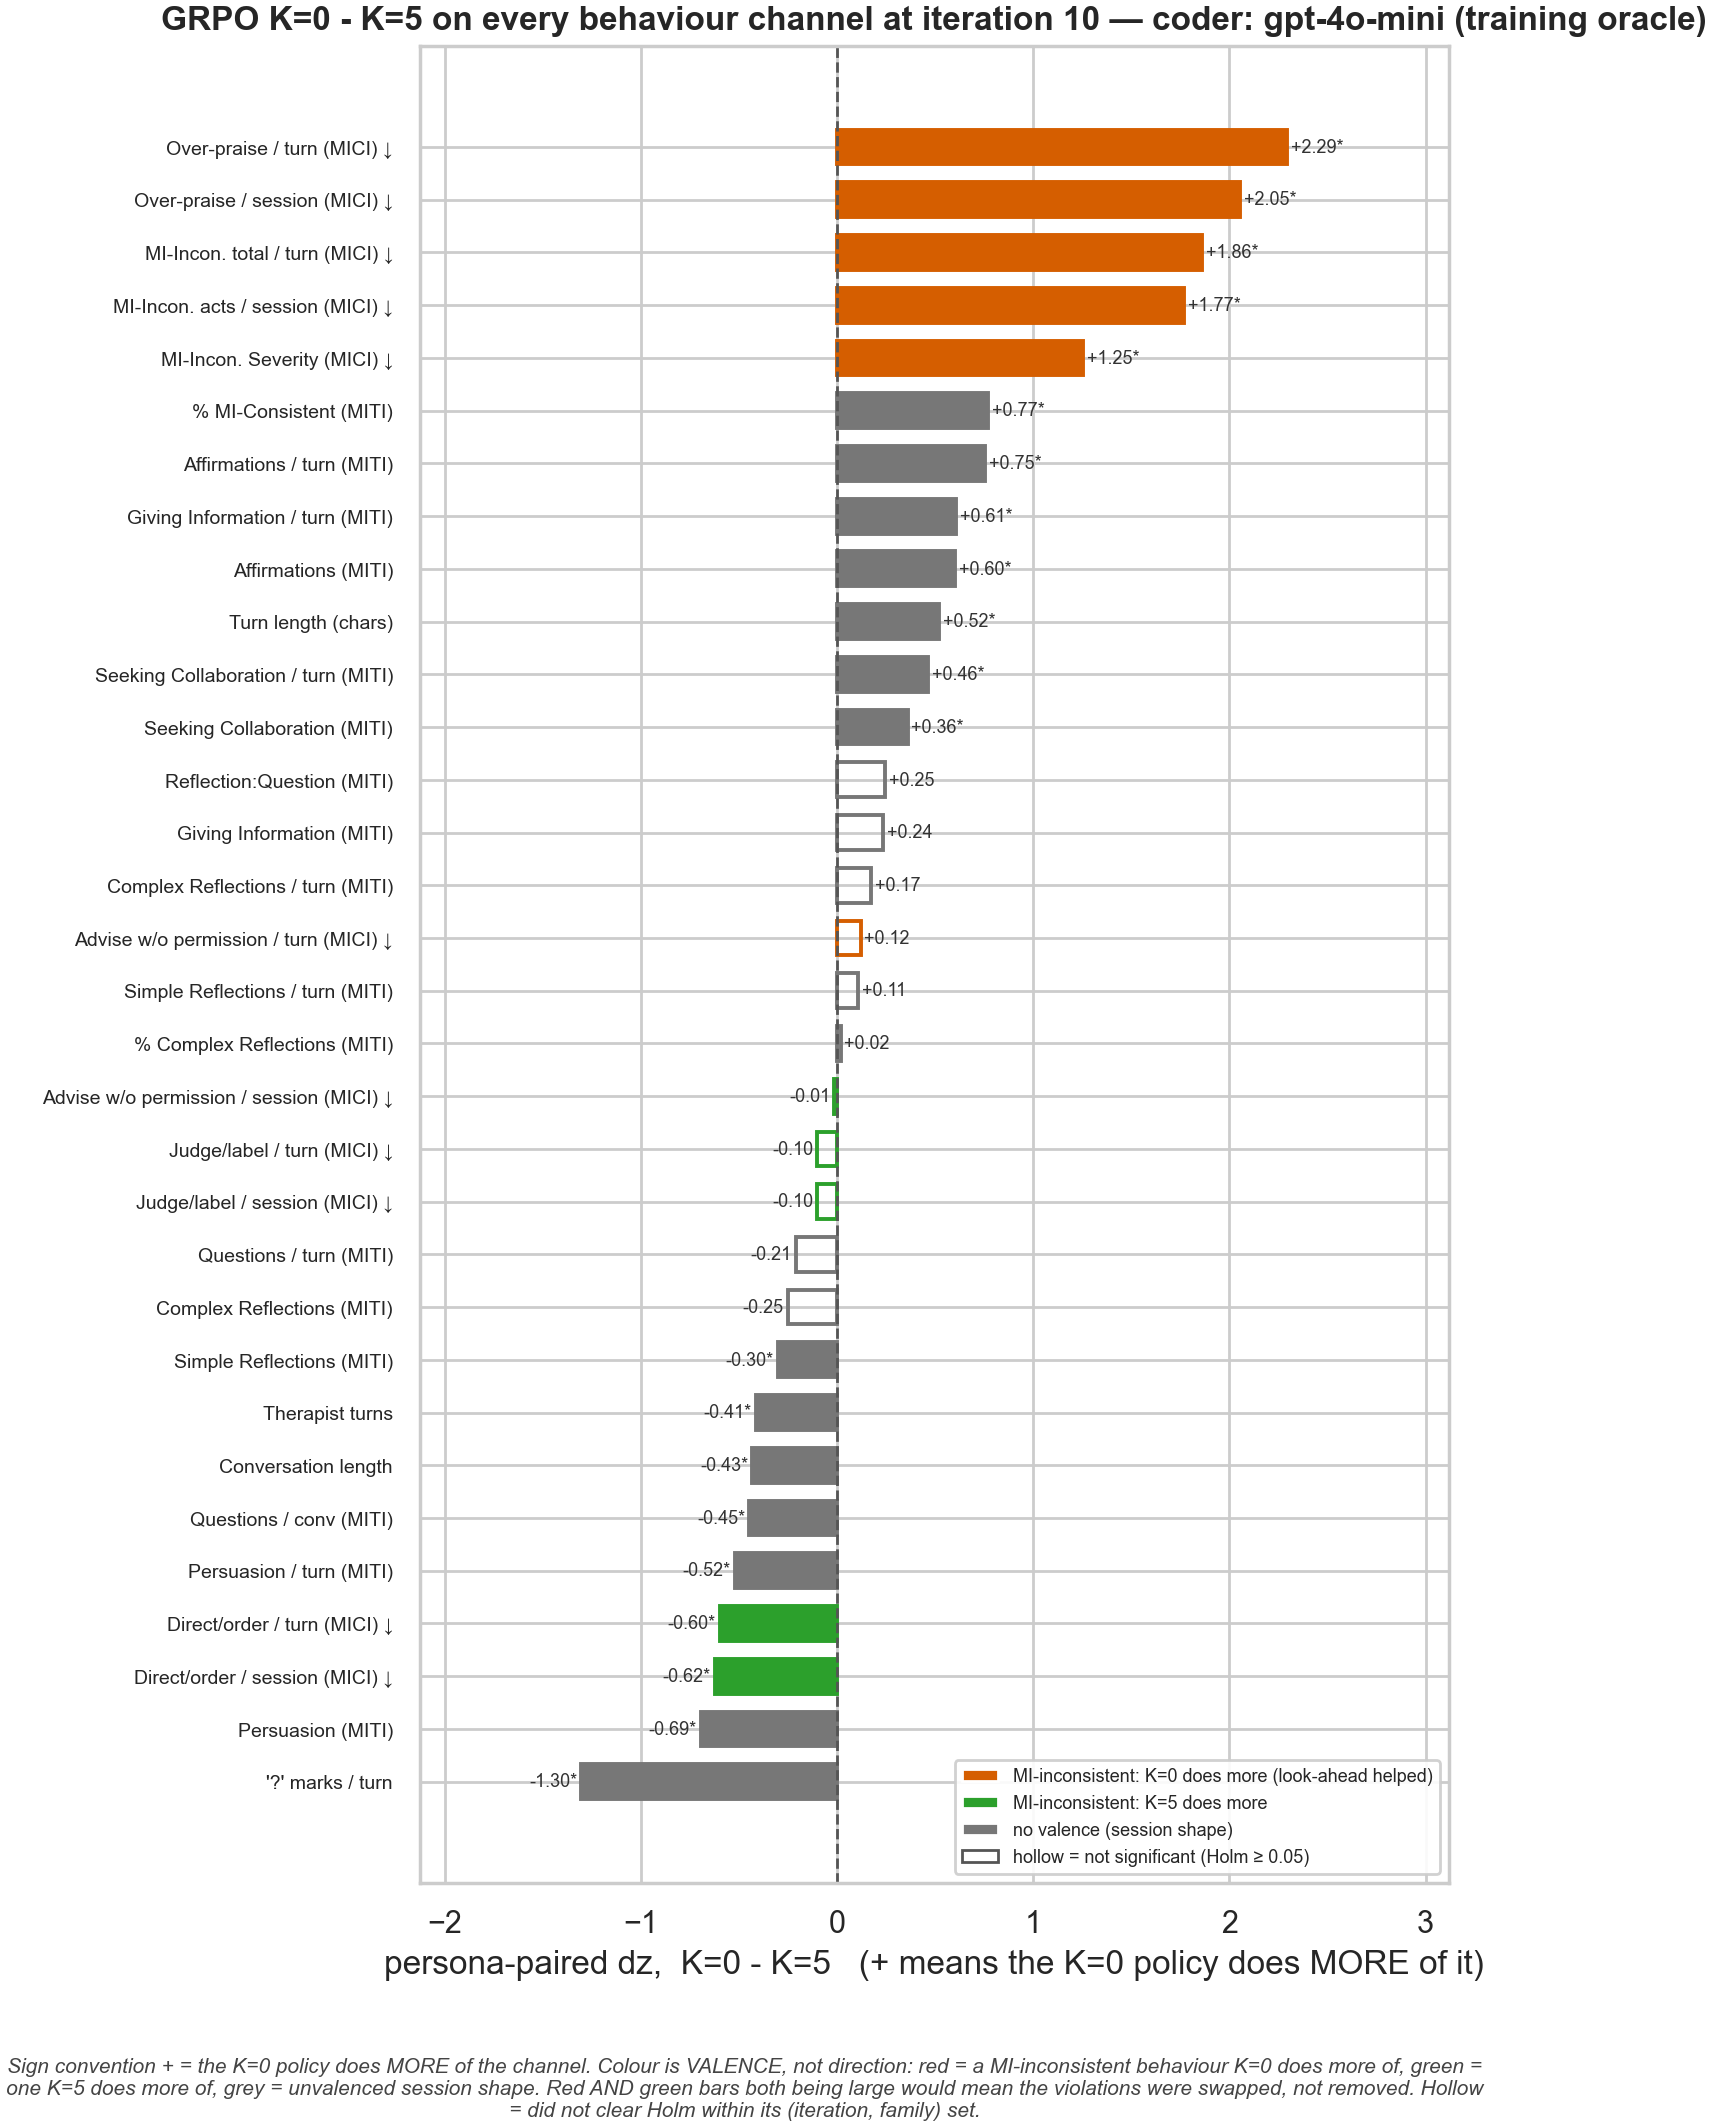
\includegraphics[width=0.85\textwidth]{figures/k_channel_forest_grpo_gpt-4o-mini.png}
\caption{\GRPO: the same frame. Over-praise dominates the $\Kz$ side and no channel of
comparable size opens on the $\Kf$ side.}
\end{figure*}
